% !TeX root = multianalysis.tex
% !TeX encoding = UTF-8
% !TeX program = XeLaTeX

\begin{frame}

\begin{tikzpicture}[overlay]
\pgfmathdeclarerandomlist{symbols}{%
  {\texttt{\string Cluster}}%
  {\texttt{\string LDA}}
  {\texttt{\string PCA}}
  {\texttt{\string Factor}}}
\foreach \y in {0,-1,...,-7} {
  \foreach \x in {0,1,...,12} {
    \pgfmathrandomitem{\randsymbol}{symbols}
    \node[black!15,rotate=45] at (\x,\y) {\randsymbol};
  }
}
\end{tikzpicture}
\titlepage
\end{frame}

\begin{frame}{本次报告所使用的分析方法}
  % \pause
    \begin{itemize}%%[<+->]
        \item 聚类分析(Cluster analysis)
        \begin{itemize}
          \item 系统聚类(Hierarchical clustering)
          \item K-means聚类(k-means clustering)
        \end{itemize}

        \item 主成分分析(Principal component analysis)

        \item 线性判别分析(Linear discriminant analysis)
        % \begin{itemize}
        %   \item Fisher 线性判别(Fisher's linear discriminant)
        %   \item Bayes 判别(Bayes discriminant)
        % \end{itemize}
    \end{itemize}
\strut
\end{frame}

\begin{frame}{本次报告所使用的数据}{某中学火箭班、实验班、重点班、普通班80名同学的期中考试成绩}
  \begin{columns}
    \column{.5\textwidth}
    \begin{figure}
      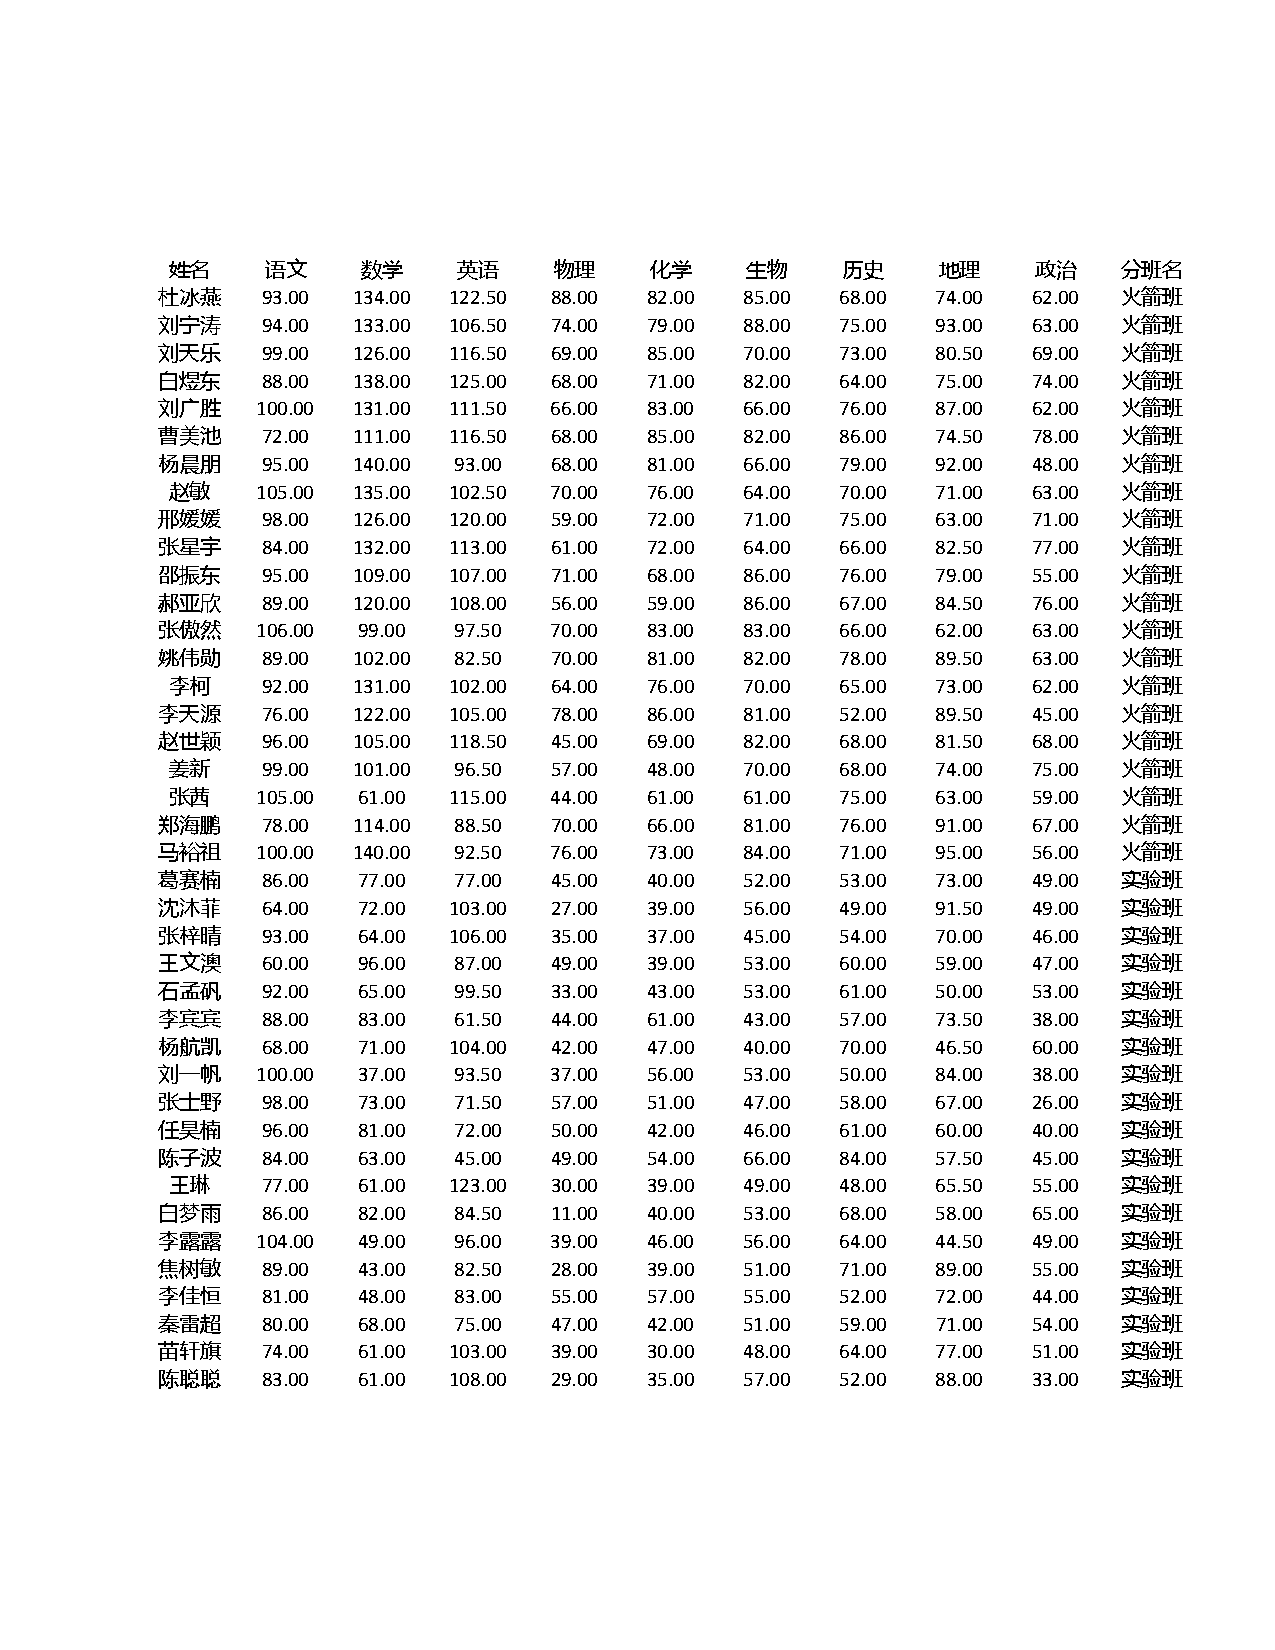
\includegraphics[height=7.7cm]{grades1.pdf}
    \end{figure}

    \column{.5\textwidth}
    \begin{figure}
      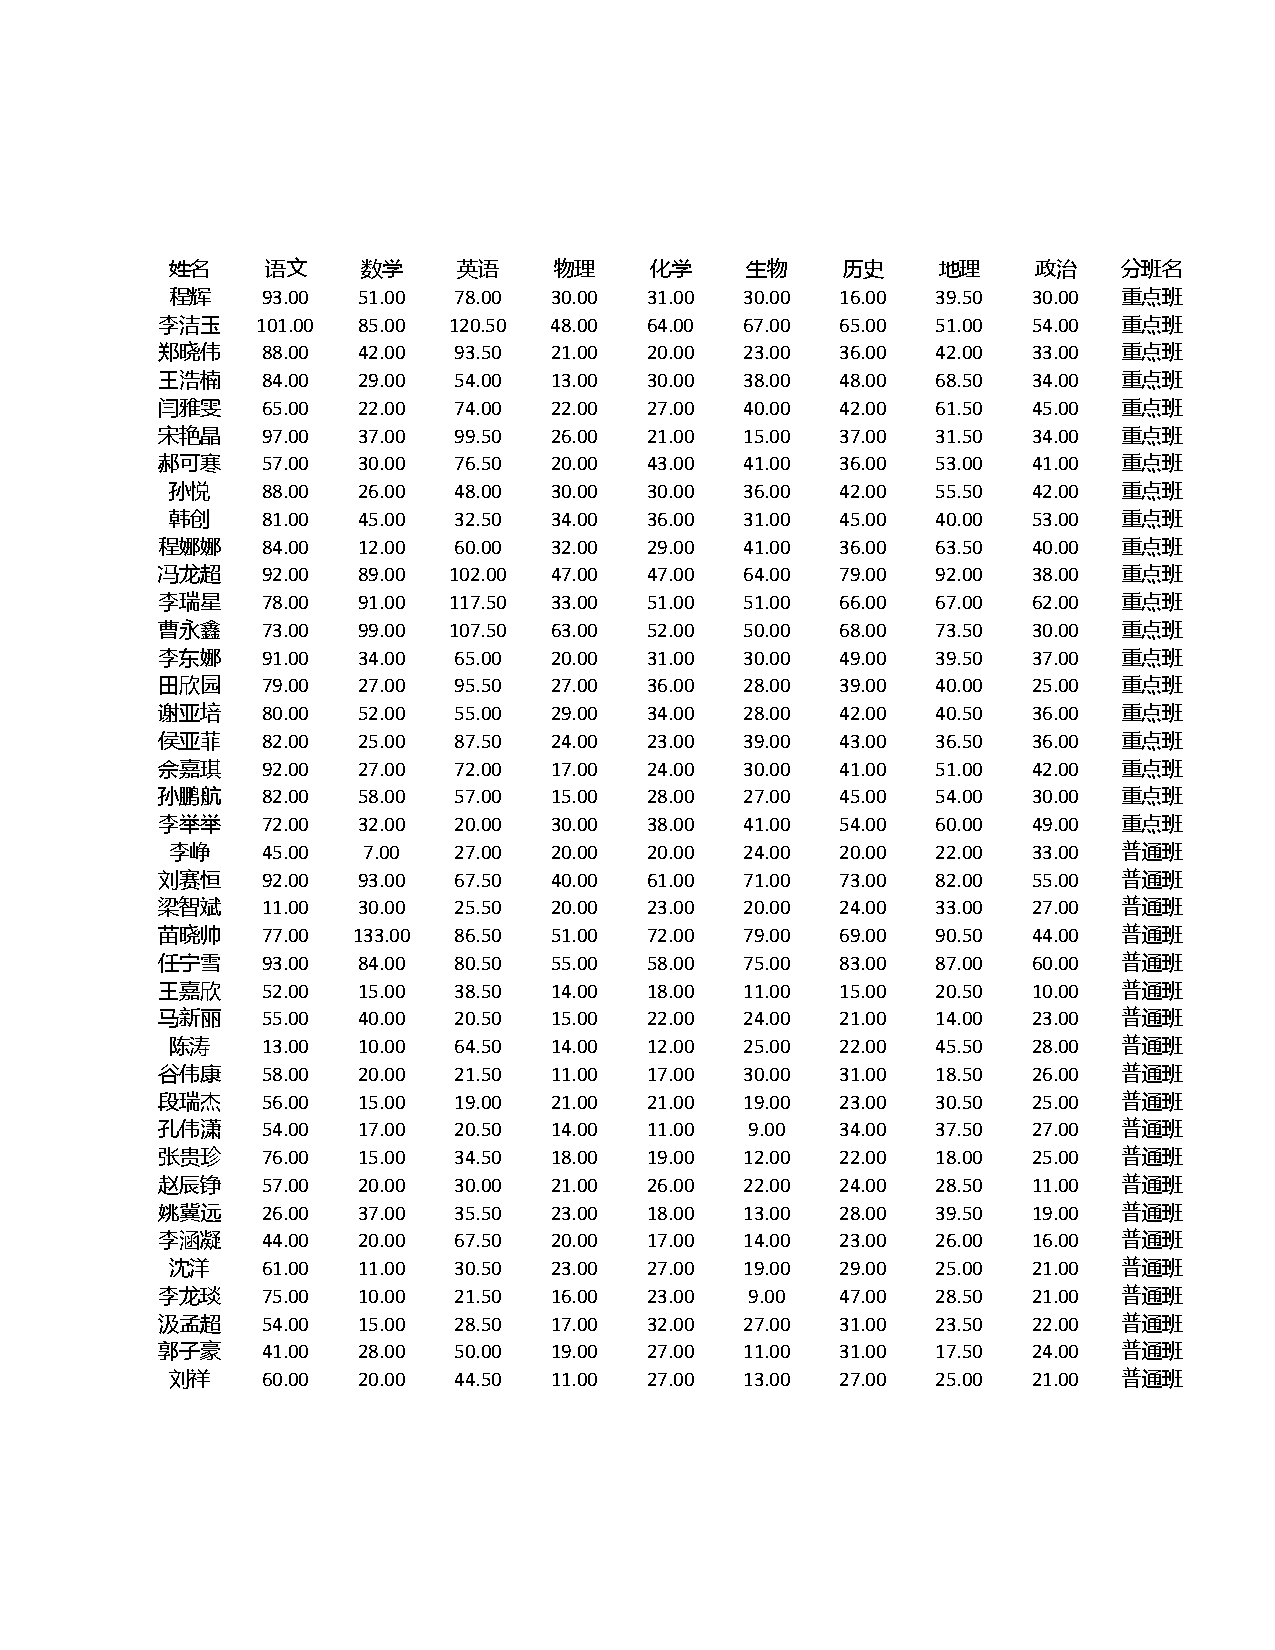
\includegraphics[height=7.7cm]{grades2.pdf}
    \end{figure}
  \end{columns}
  \strut
\end{frame}
